\documentclass{article}
\usepackage[francais]{babel}
\usepackage[utf8]{inputenc}  
\usepackage{listings}
\usepackage{graphicx}
\usepackage{color}
\usepackage{float}

% Style for c code
\definecolor{mygreen}{rgb}{0,0.6,0}
\definecolor{gray}{rgb}{0.5,0.5,0.5}
\definecolor{mymauve}{rgb}{0.58,0,0.82}
\definecolor{backcolour}{rgb}{0.95,0.95,0.92}

\lstdefinestyle{cstyle}{ 
  language=C,
  backgroundcolor=\color{backcolour},   
  basicstyle=\footnotesize,        % the size of the fonts that are used for the code
  captionpos=b,                    % sets the caption-position to bottom
  commentstyle=\color{mygreen},    % comment style
  deletekeywords={...},            % if you want to delete keywords from the given language
  escapeinside={\%*}{*)},          % if you want to add LaTeX within your code
  keepspaces=true,                
  keywordstyle=\color{blue},       % keyword style
  otherkeywords={*,...},           % if you want to add more keywords to the set
  numbers=left,                   
  numbersep=5pt,                   % how far the line-numbers are from the code
  numberstyle=\tiny\color{gray}, % the style that is used for the line-numbers
  rulecolor=\color{black},        
  showspaces=false,               
  showstringspaces=false,          % underline spaces within strings only
  showtabs=false,                  % show tabs within strings adding particular underscores
  stepnumber=1,                    % the step between two line-numbers. If it's 1, each line will be numbered
  stringstyle=\color{mymauve},     % string literal style
  tabsize=2,	                   % sets default tabsize to 2 spaces
  title=\lstname                   % show the filename of files included with \lstinputlisting; also try caption instead of title
}

\lstset{style=cstyle}

\title{Simulation de la gravitation universelle}
\author{Benjamin \bsc{Angelaud} - Adrien \bsc{Guilbaud}}
\begin{document}
\maketitle
% gregoire.pichon@inria.fr
% Deadline 5 novembre, minuit

% n particules plan 2D
% mémoire limitée par processus

% *une masse mi
% *une position vec(pt(Mi)) 
% *une vitesse vec(vt(Mi))

% \paragraph{}
% $ F_t(M_i, M_j) = F_t(M_j, M_i) * \overrightarrow{u}_{ij} $
% \paragraph{}
% $ F_t(M_i, M_j) = G \frac{m_i m_j}{(M_i M_j)^2} * \overrightarrow{u}_{ij} $
% \paragraph{}
% uij unitaire dirigé de Mi à Mj
% \paragraph{}
% $ F_t(M_i) = \sum_{i=1}^{n}  F_t(M_i, M_j) i \not= j $
% \paragraph{}
% $ \overrightarrow{a_t(M_i)} = \frac{F_t(M_i)}{m_i} $
% \paragraph{}
% Discrétitation avec un pas de temps dt: 
% $ \overrightarrow{pt+dt}(M_i) = \overrightarrow{pt}(M_i) + \overrightarrow{vt}(M_i)dt + \frac{\overrightarrow{at}(M_i)}{2} * dt^2 $
% \paragraph{}
% v(t)+dt(Mi)  =vt(Mi) + at(Mi)dt
% \paragraph{}
% Il faut fixer un dt: petit si les particules sont proches pour éviter les colissions.


\section{Version séquentielle}
Avant de commencer la version parallèle, nous avons d'abord choisi de programmer en séquentiel dans le but de pouvoir valider notre code sans que les erreurs pouvant être provoquées par MPI ne rentre en ligne de compte. De plus, le code permettant le calcul des forces pouvait être entierement réutilisé dans la version parallèle. Cela nous permet également d'avoir un bon point de comparaison pour valider les résultats en obtenus en MPI.

\subsection{L'implémentation séquentielle}
Nous avons créé une structure (fig. \ref{struct}) permettant de stocker l'état des particules (i.e. la masse, un vecteur position et un vecteur vitesse). En effet, il n'est pas nécessaire de stocker l'accéleration directement dans la structure car elle est recalculée à chaque pas de temps.

\begin{figure}[h]
  \centering
  \begin{lstlisting}[language=C]
    typedef struct particle_s{
      double m;
      double p[2];
      double v[2];
    }particle_t;\end{lstlisting}
  \caption{\label{struct}Structure d'une particule}
\end{figure}

Nous discuterons de la pertinence de ce choix dans la partie \ref{subsec:datatype}.



\subsection{Exécution séquentielle}

\begin{figure}[h]
  \centering
  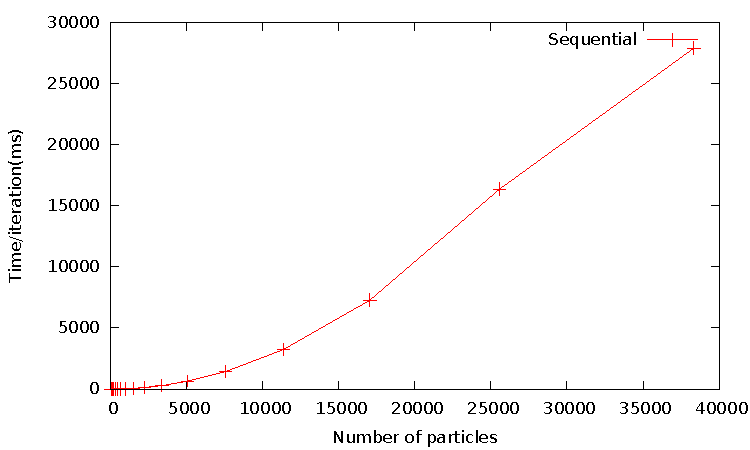
\includegraphics[scale=0.7]{ResultTDP2/seq_temps_iter/seq.pdf}
  \caption{\label{seq_ti}Temps/itération en fonction du nombre de particules}
  
\end{figure}
Nous pouvons observer sur cette courbe (fig \ref{seq_ti}) que l'algorithme a un comportement quadratique. En effet, l'algorithme utilisé est en $ O(n^2) $ car à chaque pas de temps, chaque particule doit intéragir avec les $ n-1 $ autres particules.


\section{Version MPI}
Nous avons ensuite débuté l'implémentation de la version MPI de l'application. Nous utilisons une fonction ``forces'' (utilisée dans la version séquentielle) qui permet de calculer les intéractions entre 2 ensemble de particules et de calculer le pas de temps $ dt $ qui sera utilisé.

\subsection{Structure de données MPI}
Nous nous somme ici intéressé à l'impact de la taille de la structure de données que les processus s'échangaient. Pour cela, nous avons d'abord créé un datatype MPI grace à la fonction MPI\_Type\_create\_struct contenant les mêmes données que la structure utilisé par la version séquentielle (fig \ref{struct}). Nous avons ensuite comparé les temps d'exécution de la simulation avec ce type de données et un second ne contenant pas les vitesses.

\begin{figure}[!h]
  \centering
  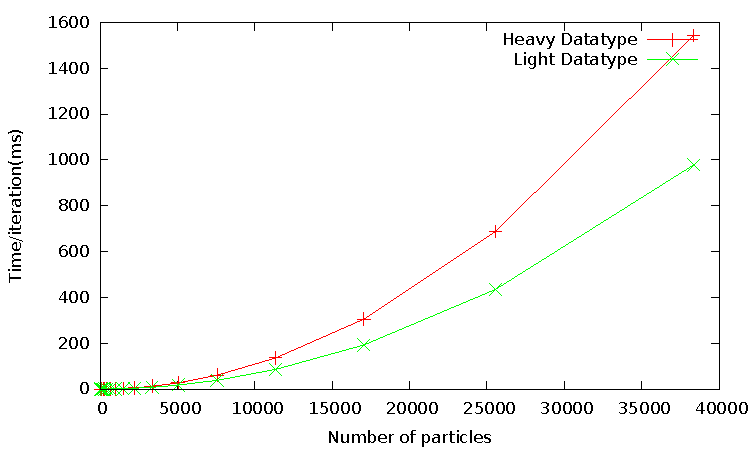
\includegraphics[scale=0.7]{ResultTDP2/mpi_datatype/mpi_datatype_singlenode.pdf}
  \caption{\label{fig:tf(n)data1}Comparaison du datatype sur 1 noeud}
\end{figure}

\begin{figure}[!h]
  \centering
  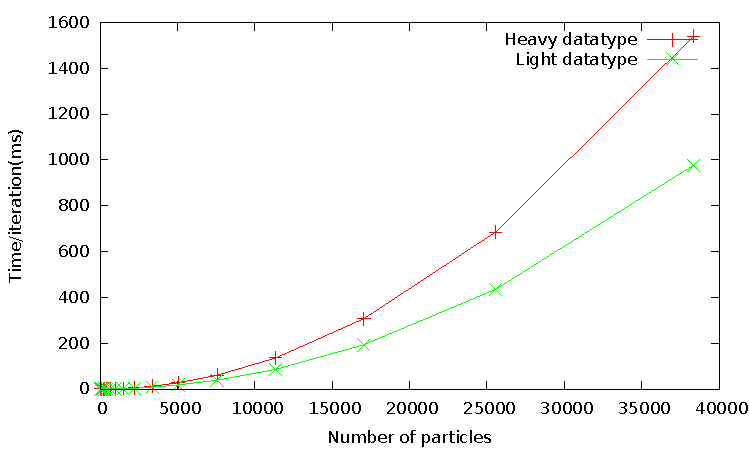
\includegraphics[scale=0.7]{ResultTDP2/mpi_datatype/mpi_datatype_multinode.pdf}
  \caption{\label{fig:tf(n)data2}Comparaison du datatype sur 2 noeuds}
\end{figure}


\paragraph{}
Sur les figures \ref{fig:tf(n)data1} et \ref{fig:tf(n)data2}, nous pouvons observer que la durée d'une itération diminue lorsque l'on n'envoie plus les vitesses des particules lors des communications inter-processus. Pour chaque itération de la simulation, $ nbProc \times (nbProc - 1) $ messages sont envoyés. Nous économisons donc l'envoi de $ nbMessages \times nbIter \times \frac{nbParticules}{nbProc} \times 2 $ double sur une exécution complète par rapport à l'autre type de donnée. Par exemple, pour 10000 particules et 1000 itérations sur 20 processus, cela représente 2,8 Go de données non-envoyées. Nous avons donc choisi de garder ce type de données pour la suite du rapport.

\newpage

\subsection{Choix des communications}
Nous nous sommes ensuite intéressé aux différents modes de communications disponibles avec MPI dans le but de comparer leurs impacts sur les performances de l'application. Dans un premier temps, nous avons utilisé les comunications point-à-point non-bloquantes. Cependant, les communications étant toujours appelées avec les mêmes arguments, il était possible de les transformer en communications persistantes.

\begin{figure}[h]
  \centering
  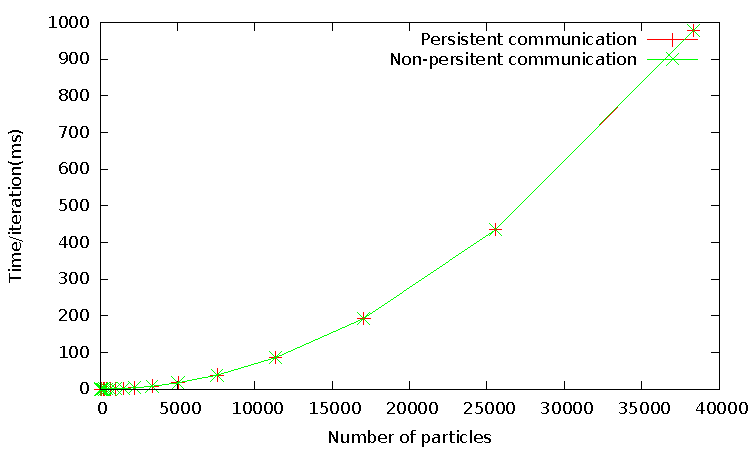
\includegraphics[scale=0.7]{ResultTDP2/mpi_comm/mpi_comm_singlenode.pdf}
  \caption{\label{fig:tf(n)1}Comparaison du type de communications sur 1 noeud}
\end{figure}

\begin{figure}[h]
  \centering
  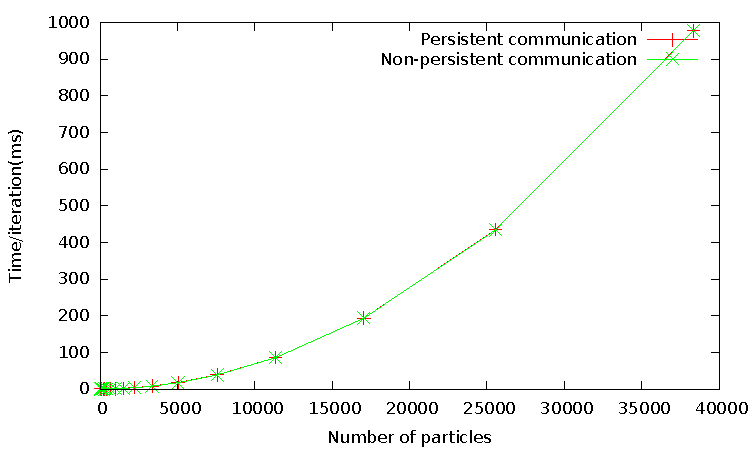
\includegraphics[scale=0.7]{ResultTDP2/mpi_comm/mpi_comm_multinode.pdf}
  \caption{\label{fig:tf(n)2}Comparaison du type de communications sur 2 noeuds}
\end{figure}


\paragraph{}
Nous pouvons observer sur les figures \ref{fig:tf(n)1} et \ref{fig:tf(n)2} que le fait d'utiliser des communications persistantes ou non ne semble pas avoir d'influence sur la durée d'exécution d'une itération que ce soit sur un seul ou deux noeud NUMA. Cela peut être expliquer par le fait que les calculs recouvrent les communications. Nous avons donc voulu profiler notre application pour en être sûr mais nous n'avons pas trouvé les outils nécessaires sur PlaFRIM.




\section{Procédure de test}
Pour réaliser l'ensemble des courbes présentées, nous avons utilisé la même procédure. Que ce soit dans la version séquentielle ou la version paralléle, nous mesurons seuleument le temps pris pour calculer l'ensemble des intéractions puis la mise à jour des positions et des vitesses. En MPI, ce temps prend en compte le temps des communications. Nous avons choisi de mesurer le temps d'une itération en fonction du nombre de particules car c'est une unité de temps suffisante pour étudier le comportement de la simulation. Tout les tests sont effectués sur 24 coeurs sur PlaFRIM: 
\begin{itemize}
\item 1 noeud NUMA, 24 coeurs;
\item 2 noeuds NUMA, 12 coeurs/noeud.
\end{itemize}

Pour générer les courbes nous mesurons donc le temps d'exécution d'une itération pour un nombre de particules variant de 24 à environ 40000 par pas de 50\%.

\section{Comparaison}

\begin{figure}[h]
  \centering
  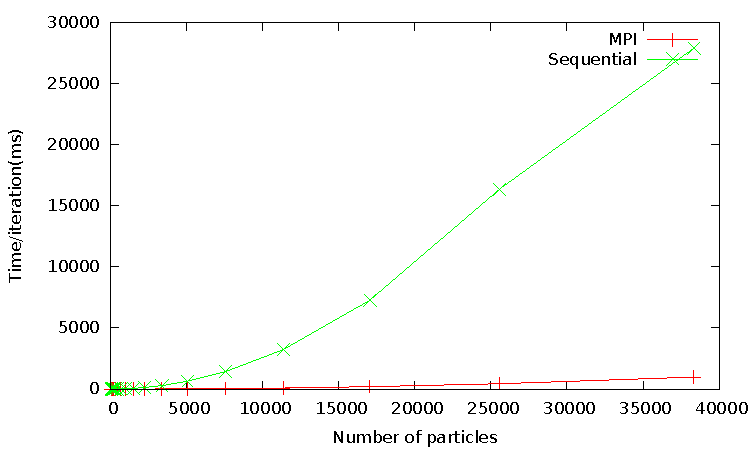
\includegraphics[scale=0.7]{ResultTDP2/seq_mpi.pdf}
  \caption{\label{seq_mpi}Comparaison MPI/séquentielle}
\end{figure}



\section{Améliorations possibles}
\subsection{Algorithmique}
Afin d'améliorer les performances de cette application, nous pourions éviter de calculer les interactions entre toutes les particules. En effet, la force gravitationnelle étant inversement proportionnelle à la distance au carré, elle devient négligeable pour des particules trés éloignées. Au lieu de découper le tableau contenant les particules, nous pourrions diviser l'espace en une grille (fig \ref{algobloc}). Chaque bloc ainsi obtenu ne devrait intéragir qu'avec lui même et les 8 blocs adjacents. Ceci réduirait le temps de calcul des intéractions ainsi que la quantité de données échangée par les processus MPI.

\paragraph{} 
Il faut par contre pouvoir déterminer la taille de ces blocs afin de ne pas complétement fausser les résultats. 

\begin{figure}[ht]
  \centering
  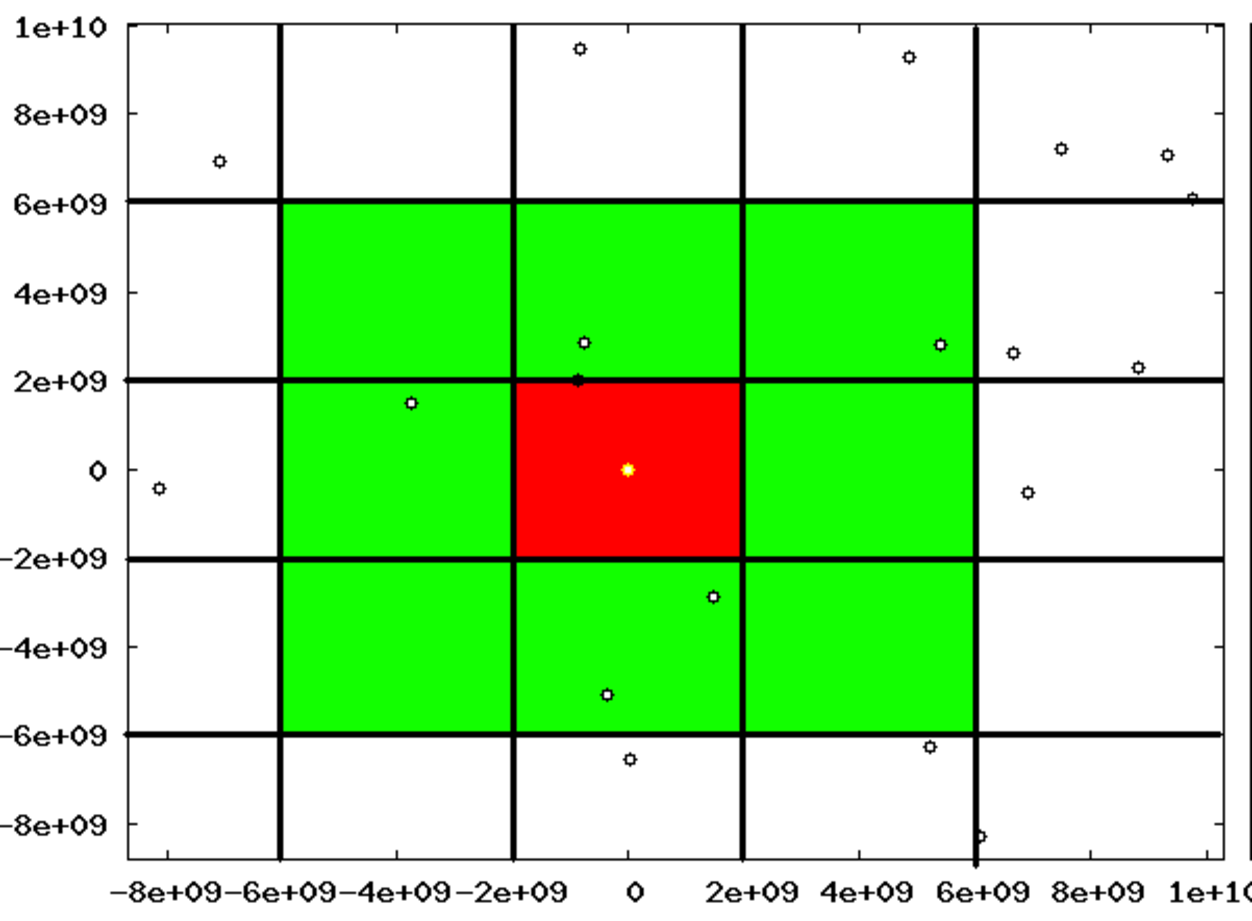
\includegraphics[scale=0.5]{ResultTDP2/algobloc.pdf}
  \caption{\label{algobloc}Algorithme par bloc - Division de l'espace}
\end{figure}

\subsection{Type de données}
\label{subsec:datatype}
Dans notre implémentation, nous utilisons un type de données Array of Structures (AoS). Lors du calcul des intéractions, toutes les données relatives aux particules sont chargées dans le cache, même la vitesse qui n'est pas nécessaire. Il serai donc possible d'utiliser un type de données Structure of Arrays (SoA) pour éviter que le cache soit pollué par des données inutiles.

\end{document}
